\section{Bayesian linear regression}

\subsection{Linear regression revisited}
\begin{itemize}
\item Suppose that we have data $D=\{(\xx_1, t_1), \ldots, (\xx_N, t_N) \}$
\item We assume that the data can be modelled by some function $t_n \approx y(x, \omega)+ \epsilon$, where $\epsilon$ models additive noise.
\item  We assume that noise is independent, identically distributed and Gaussian: 
\begin{align}
	\epsilon &\sim \mathcal{N}(0,\beta^{-1})\\
	t|\xx, \omega, \beta &\sim \mathcal{N}(y(\xx,\omega), \beta^{-1})
\end{align}
\end{itemize}

\begin{figure}
	\centering
	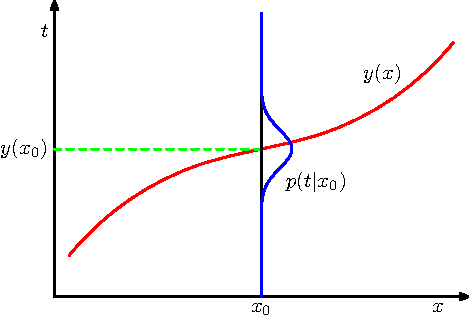
\includegraphics[width=.5\textwidth]{./lecture5/Figure128.pdf}
	\caption{Linear regression. Bishop PRML Figure 1.28}
\end{figure}


\subsection{Maximum likelihood estimation for linear regression}
\begin{itemize}
\item We consider a linear model $y(\xx,\omega)= \omega^\top \xx$
\item ~[On board: Likelihood, Maximum Likelihood Solution, Predictive distribution from MLE]\\
\item  For a Bayesian treatment, we need priors.
\end{itemize}

\begin{bbbox}{Maximum likelihood estimation for linear regression}
	\begin{align*}
			L(t | x,\omega) &= \log \left( \prod_{n=1}^N p(t_n |  x_n, \omega ) \right) \\
			        &= \sum_{n=1}^N \log \left( \frac{1}{\sqrt(2\pi)} \exp \left( - \frac{\beta}{2} \left( t_n - 	\omega^{\top} x_n \right)^2 \right) \right) \\
			        &= const. + \sum_{n=1}^N - \frac{\beta}{2} \left( t_n - \omega^{\top} x_n \right)^2 \\
			        &= const - \underbrace{\frac{\beta}{2} \sum_{n=1}^N \left( t_n - \omega^{\top} x_n \right)^2}_{AMSE - average mean squared error} \\
	   \hat{\omega} &= \left( \sum_{n=1}^N x_n x_n^{\top} \right)^{-1} \left( \sum_{n=1} x_n t_n \right) \\			 	    \end{align*}
	Predictive distribution \\
	$P(t^{*} | x^{*},0) = P(t^{*} | x^{*},\hat{\omega}) = \mathcal{N}(\omega^{\top} x^{*}, \frac{1}{\beta})$ 
\end{bbbox}

\subsection{Maximum a posteriori estimation for the linear regression.}
\begin{align}
\omega_i &\sim \mathcal{N}(0,\alpha^{-1})\\
p(\omega| \alpha) &= \prod_{i=1}^M  \sqrt{\frac{\alpha}{{2\pi}}}\exp\left( -\frac{\alpha}{2}  {\omega_i^2}\right)\\
&%
 =\left(\frac{\alpha}{2\pi}\right)^{M/2} \exp \left(-\frac{\alpha}{2} \omega^\top \omega  \right) \\
 \text{where } \forall i,j: \alpha_i &= \alpha_j
\end{align}

\begin{bbbox}{Finding the maximum-a-posteriori of $\omega$}
	\begin{align*}
		L_{post}(t | x,\omega) &= \log \left( \prod_{n=1}^N p(t_n |  x_n, \omega ) p(\omega|\alpha)\right) \\
		 &= \sum_{n=1}^N \log \left( \frac{1}{\sqrt(2\pi)} \exp \left( - \frac{\beta}{2} \left( t_n - 	\omega^{\top} x_n \right)^2 \right) \frac{\alpha}{2\pi}^{\frac{M}{2}} \exp \left( -\frac{\alpha}{2} \omega^{\top}\omega \right) \right) \\
		 &= const. - \frac{\beta}{2} \sum_{n=1}^N \left( t_n - \omega^{\top} x_n \right)^2 -\frac{\alpha}{2} \omega^{\top}\omega \\
	\hat{\omega} &= \left( \sum_{n=1}^N x_n x_n^{\top} + \frac{\alpha}{\beta} \mathbf{I}_M \right)^{-1} \left( \sum_{n=1} x_n t_n \right) \\			 
	\end{align*}
\end{bbbox}


\subsection{Basis functions in linear regression}
\textbf{If you are smart about choosing good basis functions ('features'), linear regression can get you pretty far.}
\begin{itemize}
\item If we use nonlinear basis functions $\phi(x)$, can model nonlinear relationships with $y(\omega, \xx)= \omega^\top \phi(x)$.
\item Polynomial regression: $\phi(x)=(1,x,x^2,x^3)$ ; (cubic feature space) 
\item 'Gaussian bumps': $\phi_i(x)= \exp\left((x-s_i)^2/\sigma_i^2 \right)$
\item Sigmoids $\phi_i(x)=1/(1+\exp(-x-s_i))$
\item  'Kernel methods' are essentially linear algorithms which take one basis function per data-point.
\item Predictive Mean [on board]
\end{itemize}

\begin{figure}
\centering
	\begin{subfigure}[b]{0.3\textwidth}
                \centering
                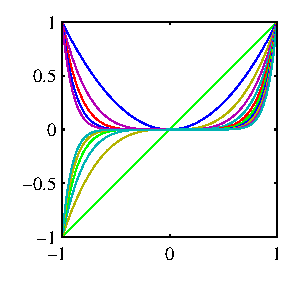
\includegraphics[width=\textwidth]{./lecture5/Figure31a.pdf}
                \caption{Polynomial basis.}
    \end{subfigure}%
	~
	\begin{subfigure}[b]{0.3\textwidth}
                \centering
                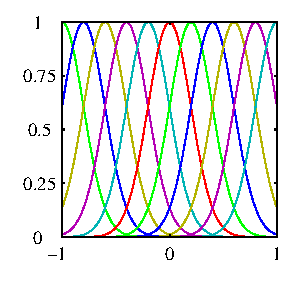
\includegraphics[width=\textwidth]{./lecture5/Figure31b.pdf}
                \caption{Gaussian bumps.}
    \end{subfigure}%
	~
	\begin{subfigure}[b]{0.3\textwidth}
                \centering
                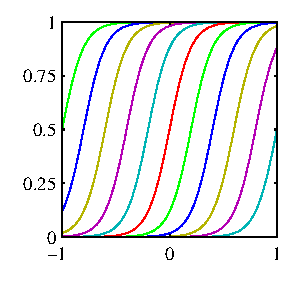
\includegraphics[width=\textwidth]{./lecture5/Figure31c.pdf}
                \caption{Logistic sigmoids.}
    \end{subfigure}%
    \caption{Non-linear basis functions, taken from Bishop PRML}
\end{figure}


\subsection{Bayesian linear regression}


\textbf{Bayesian linear regression takes into account our uncertainty about parameters.}

\begin{itemize}
\item Posterior distribution is Gaussian $\rightarrow$ Posterior mean and MAP coincide!
\item  However, neither the MLE nor the MAP solution take into account that we have (posterior) uncertainty about the parameters
\end{itemize}


\begin{figure}
\centering
	\begin{subfigure}[b]{0.45\textwidth}
		\centering	
		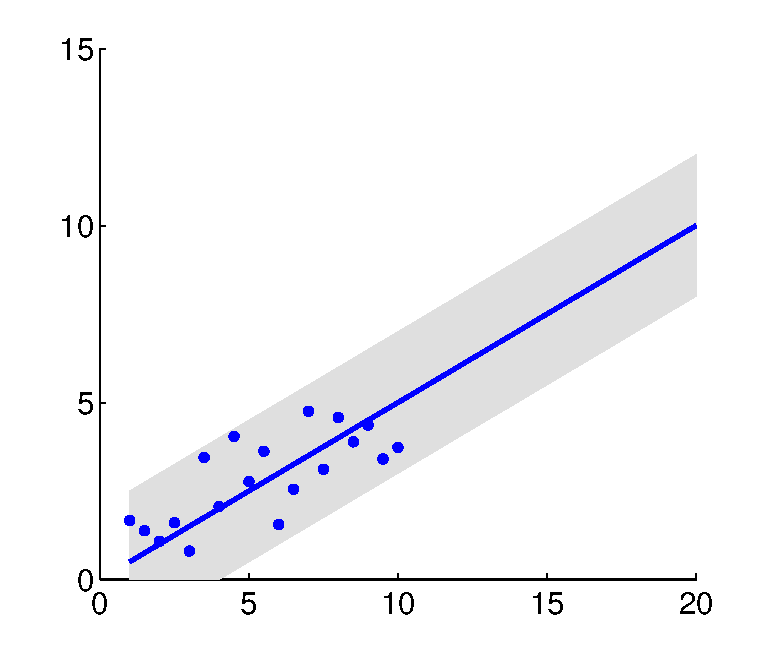
\includegraphics[width=\textwidth]{./lecture5/LinReg.pdf}
	\end{subfigure}
	~
	\begin{subfigure}[b]{0.45\textwidth}
		\centering
		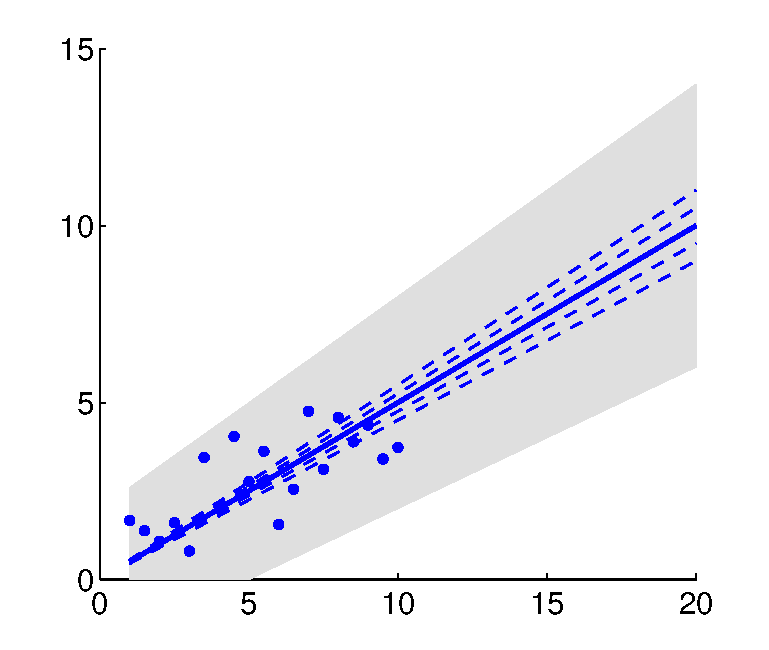
\includegraphics[width=\textwidth]{./lecture5/LinRegBayes.pdf}
	\end{subfigure}
\end{figure}


\subsection{Gaussian processes}
\textbf{Illustration: Climate prediction [by Carl Rasmussen, University of Cambridge, using Gaussian Processes]}

\begin{figure}
	\centering
	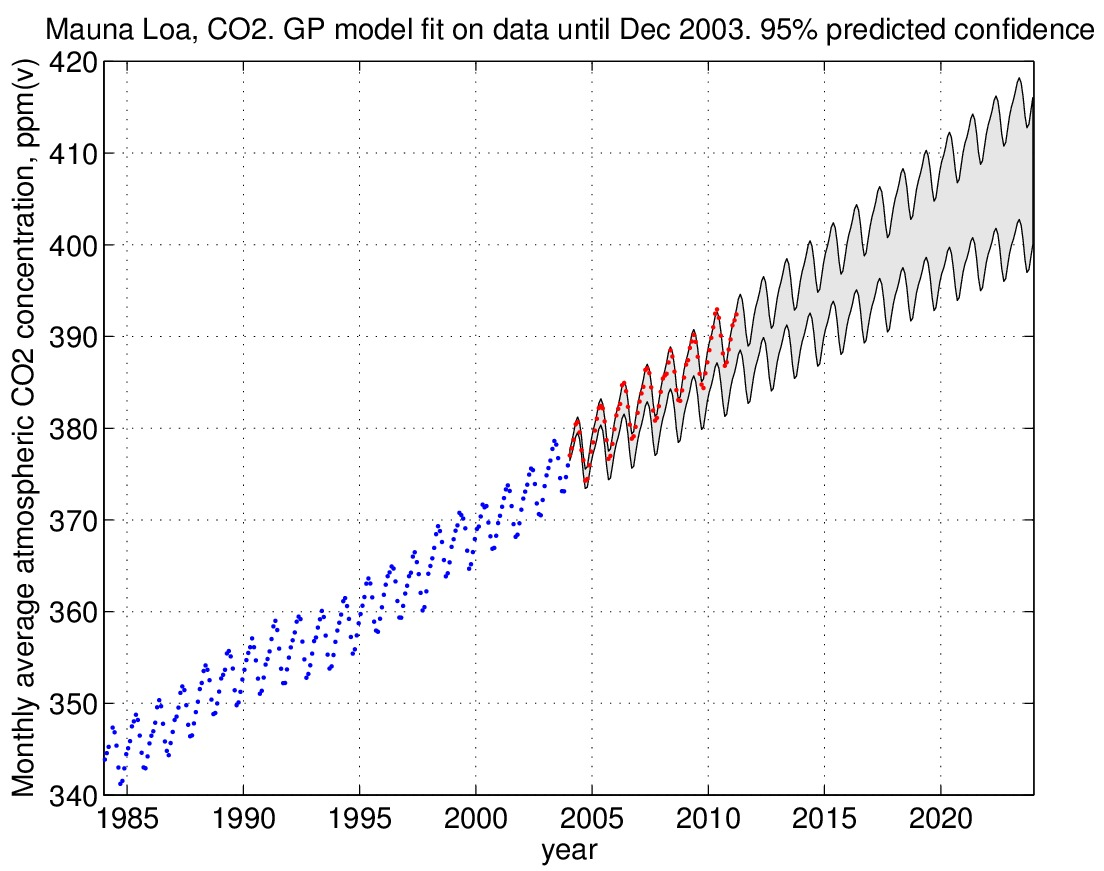
\includegraphics[width=0.5\textwidth]{./lecture5/Rasmussen2}
	\caption{Gaussian process regression.}
\end{figure}


\subsection{Sequential update of the posterior distribution}
\textbf{Bayesian regression illustrated: The more data we observe, the more constrained the parameters are.}

\begin{figure}
	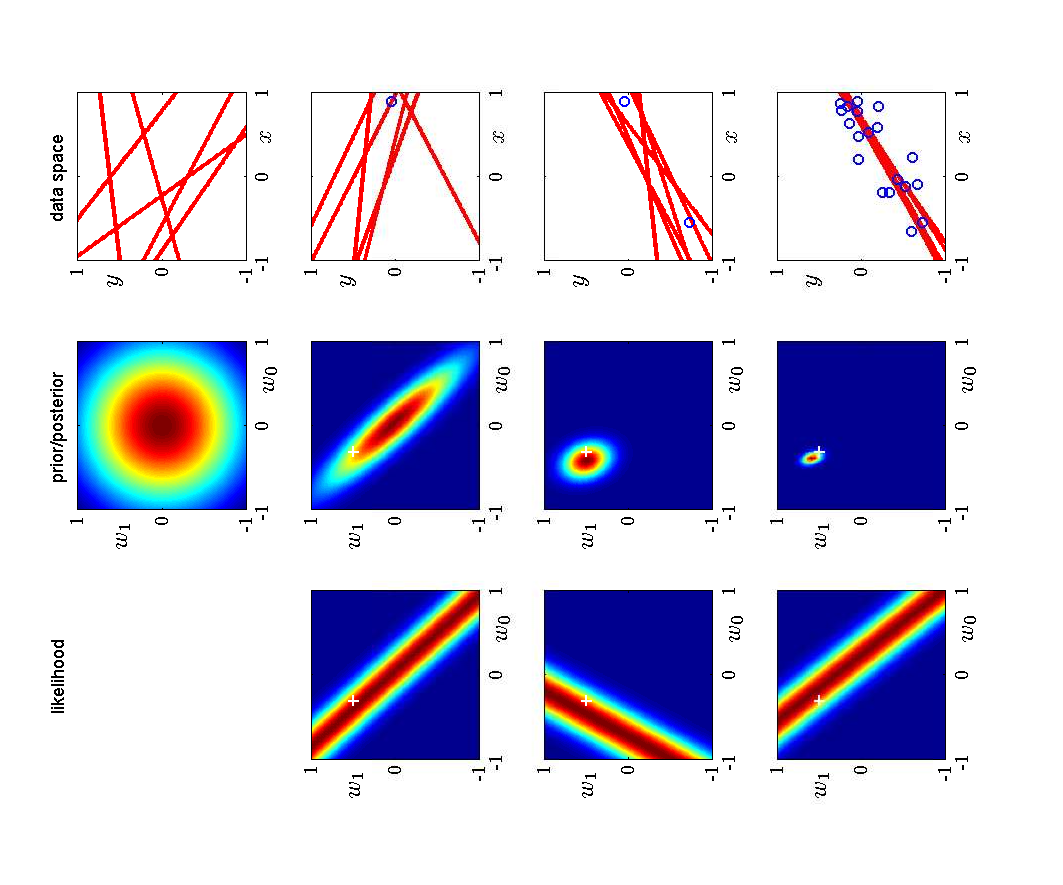
\includegraphics[width=\textwidth]{./lecture5/Figure37.pdf}
	\caption{Sequential update of the Gaussian posterior, figures taken from Bishop PRML}
\end{figure}



\textbf{Calculating the predictive mean and variance for Bayesian regression}

Assume $\alpha$ and $\beta$ as given.\\ Posterior distribution: [derivation on board]

\begin{bbbox}{Bayesian linear regression: calculating posterior mean and variance}
	Recall the quadratic form for the Gaussian: \\
	\begin{align*}
		&\frac{1}{Z} \exp \left( -\frac{1}{2} \left( x-\mu \right)^{\top} \Sigma^{-1} \left( x-\mu \right) \right) \\
		           &= \frac{1}{Z} \exp \left( -\frac{1}{2} \left( x^{\top}\Sigma^{-1}x + \mu^{\top}\Sigma^{-1}\mu 
		             - \mu^{\top}\Sigma^{-1}x - x^{\top}\Sigma^{-1}\mu \right) \right)\\
		           &= \frac{1}{Z} \exp \left( -\frac{1}{2} x^{\top}\Sigma^{-1}x + x^{\top}\Sigma^{-1}\mu + const. \right) \\
	\end{align*}
	Here again we can easily read out the posterior mean and covariance from the two terms. \\
	We say that $\omega | D \sim \mathcal{N}\left( \mu_{post}, \Sigma_{post}\right)$. \\
	Since the mode and mean of a Gaussian are the same thing we already know from our MAP estimation that:
	$ \mu_{post} = \left( \sum_{n=1}^N x_n x_n^{\top} + \frac{\alpha}{\beta} \mathbf{I}_M \right)^{-1} \left( \sum_{n=1} x_n t_n \right)$ \\
	The next thing we have to do is to bring the posterior  distribution into the quadratic form from above and to read out the posterior covariance. Note that all terms that are independents from $\omega$ will sucked into the constant term: \\
	\begin{align*}
		P(\omega|D) &= \frac{1}{Z_1} \prod_{n=1}^N P(t_n|x_n,\omega) P(\omega) \\
		&= \frac{1}{Z_2} \exp \left( \sum_{n=1}^N -\frac{\beta}{2} \left( \omega^{\top} x_n - t_n \right) ^2 - \frac{\alpha}{2} \omega^{\top} \omega \right) \\
		&= \frac{1}{Z_2} \exp \left( -\frac{\beta}{2} \sum_{n=1}^N \left( \omega^{\top} x_n - t_n \right) \left( \omega^{\top} x_n - t_n \right)^{\top} - \frac{\alpha}{2} \omega^{\top} \omega \right) \\
		&= \frac{1}{Z_3} \exp \left( -\frac{1}{2} \left( \beta \sum_{n=1}^N \omega^{\top} x_n x_n^{\top} \omega + \alpha \omega^{\top} \omega \right) \right) \\
		&= \frac{1}{Z_3} \exp \left( -\frac{1}{2} \left( \omega^{\top} \left( \beta \sum_{n=1}^N x_n x_n^{\top} + \alpha \mathbf{I}_M \right) \omega \right) \right) \\
		\Sigma_{post}^{-1}&=\alpha \mathbf{I}_M + \beta \sum_{n=1}^N x_n x_n^\top\\
	\end{align*}
\end{bbbox}

\begin{align}
\Sigma_{post}^{-1}&=\alpha \mathbf{I}+\beta \sum_i x_i x_i^\top\\
\mu_{post}&=\Sigma_{post} \beta \sum_i x_i t_i
\end{align}

Predictive distribution: [derivation on board]

\begin{bbbox}{Predictive distribution}
	We note that in the case of a regression the predictive error arises from our uncertainty about the parameters as well as the variance which is inherent to our predicted variable. We want to calculate the predictive distribution starting from the observation that making a prediction is basically a concatenation of two random variables.
	\begin{align*}
		t^* &| D, x_*: \;
		t^* = \underbrace{\omega^{\top}x_*}_{y^*} + \epsilon \\		
%		\mu &\sim \mathcal{N}(\mu_0, \frac{1}{\tau}); \;
%		x|\mu \sim \mathcal{N}(\mu,\frac{1}{\beta}); \;
%		\rightarrow x \sim \mathcal{N}(\mu_0, \frac{1}{\tau} + \frac{1}{\beta}) \\
		y^* &\sim \mathcal{N} (\mu_*,\frac{1}{\tau_{*}}); \;
		t^*|y^* \sim \mathcal{N}(y^*,\frac{1}{\beta}); \;
		\rightarrow \underbrace{t^* \sim \mathcal{N}(\mu_*,\frac{1}{\tau_{*}} + \frac{1}{\beta})}_{\text{Predictive distribution}} \\
	\end{align*}
	
We see that the variance of our predictive distribution is calculated from the variance in our parameter estimate and from the variance in $t$. We can further express the posterior distribution based on:
	\begin{align*}
		\mu_* &= E(y^* | D) = E(\omega^{\top} x_* | D) \\
		      &= E(\omega^{\top} | D) x_* = E(\omega | D)^{\top} x_* \\
		      &= \mu_{post}^{\top} x_* \\
		\frac{1}{\tau_{*}} &= \mbox{Var}(y^* | D) \\
		     &= \mbox{Var}(\omega^{\top} x_* | D) = x_*^{\top} \mbox{Var}(\omega^{\top} | D) x_* \\
   		     &= x_*^{\top} \Sigma_{post} x_* \\
	\end{align*}
\end{bbbox}

\begin{align}
E(t^*|D,x^*)&= \mu_{post}^\top x^* \\
\mbox{Var}(t^*|D,x^*)&=  1/\beta+ x^{*\top} \Sigma_{post} x^*
\end{align}
What if there are basis functions? [on board]



\subsection{Fully Bayesian linear regression}


\textbf{But, where do we get $\alpha$ and $\beta$ from?}

\begin{itemize}
\item Bad news: Getting these makes things more complicated.
\item  Good news: This will not be on the exam (unless I take that back explicitly...). 
\item  'Full' Bayesian inference: Integrate out $\alpha$, $\beta$. No closed form solution. Use (e.g.) variational inference.
\item  Practical solution: optimize $\alpha$ and $\beta$ by \emph{maximizing the evidence}, also known as \emph{marginal likelihood} or \emph{likelihood type 2}
\begin{align}
E&=\log P(\alpha, \beta|D)\\
&= \log \int_\omega p(D|\omega,\beta) p(\omega|\alpha) p(\alpha,\beta)    d \omega\\
&= \frac{M}{2}\log(\alpha)+\frac{N}{2}\log \beta-\mbox{M}(\mu_{post})+\frac{1}{2}|\Sigma_{post}|-\frac{N}{2} \log(2\pi) 
\end{align}
\item $\mu_{post}$ and $\Sigma_{post}$ are the posterior mean and covariance, and $\mbox{M}(\mu_{post})=\frac{\beta}{2}\sum_n (t_n-y(\mu_{post},\xx_n))^2+\frac{\alpha}{2} \mu_{post}\mu_{post}^\top$ is the quadratic cost function evalulated at the posterior mean (see Bishop 3.5 for details).
\end{itemize}


\textbf{Optimization of the marginal likelihood is a Bayesian alternative to parameter-setting by cross-validation.}

\textbf{What we have not had time to cover:}
\begin{itemize}
\item \emph{Non-Gaussian priors:} The most important non-Gaussian prior is the `Laplace prior' ('L1 regularization'), which leads to sparse MAP-solutions.
\item \emph{Non-Gaussian noise models:} If you know that your noise is not Gaussian but, say, Poisson, use 'generalized linear regression'. Some choices of noise models are more robust to outliers than the Gaussian. We will do one specific example of generalized linear regression in the last lecture.
\item \emph{Nonlinear regression models:} The most important Bayesian nonlinear regression technique is \emph{Gaussian process regression}. In a nutshell, GP regression is like linear regressions but the algorithm puts ne basis function at each data-point. To understand GP regression, you need to understand Gaussians.
\end{itemize}


